\chapter{Descripción de los problemas en fluidos con transferencia de calor }
\graphicspath{{figs/cap4/}}
\label{cap4}

En el presente capíulo se realiza la descripción de los problemas con transferencia de calor para fluidos multifásicos con cambio de fase llevados a cabo para validar los códigos numéricos desarrollados, siendo éstos la \textit{Construcción de Maxwell}, la \textit{Estratificación de un fluido Van Der Waals con temperatura no uniforme} y la \textit{Generación de burbujas en una superficie horizontal calefaccionada}.

\section{Construcción de Maxwell}

Como se desarrollo en el Cap. \ref{cap2} la Ec. (\ref{eq:VdW_P}) es una EOS que modela el comportamiento de un gas real.

\begin{align*}
	p = \frac{R T}{V_m - B} - A {\left(\frac{1}{V_m}\right)}^2
\end{align*}

La Ec. (\ref{eq:VdW_P}) puede ser representada gráficamente en un diagrama $P - V_m$. \\ La Figura \ref{fig:P_V_CO2} muestra el diagrama mencionado para el dióxido de carbono ($CO_2$) a distintas temperaturas: 373 (K), 304 (K) y 270 (K). Para $T = 270 \> K$ se vislumbra que en $p = 44,08 \> atm$ la gráfica se intersecta en tres valores de $V_m$, siendo dos de ellos estables; por lo que se observa que hay dos volúmenes molares de coexistencia, indicando las fases líquido y gaseosa.

La construcción de Maxwell, también llamada regla de igualdad de áreas, indicada en Ec. (\ref{eq:maxwell_Construction}), es un procedimiento analítico para encontrar las densidades de coexistencia del líquido y gas. Donde $P$ es la presión de la EOS y $p_0$ es una presión constante. Al realizar la integral propuesta surge que las áreas \textbf{A1} y \textbf{A2} de la Figura \ref{fig:P_V_CO2} deben ser iguales.

\begin{equation}
\int_{V_{m,l}}^{V_{m,g}} P d V_m = p_0 (V_{m,l} -  V_{m,g})
\label{eq:maxwell_Construction}
\end{equation}

\begin{figure}[h!]
	\centering
	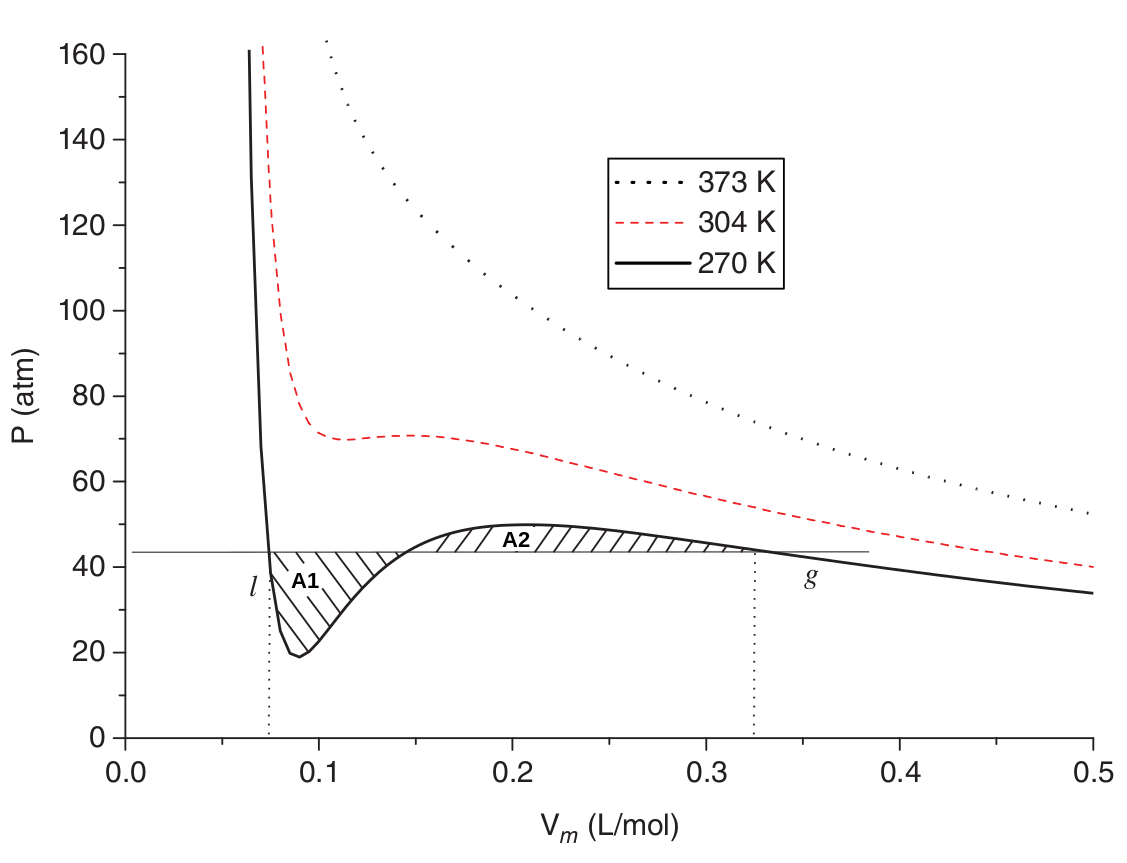
\includegraphics[width=.8\textwidth]{figs/cap4/Diagrama_P_V_del_CO2_Multiphase_LBM}
	\caption{Diagrama $P - V_m$ de la EOS de VdW del $CO_2$ con las constantes $a = 3,592$ y $b = 0,04267$, representando par a $T = 270 \> K$ los volúmenes molares del líquido y gas. \cite{huang2015multiphase}}
	\label{fig:P_V_CO2}	
\end{figure}


La Ec. (\ref{eq:VdW_P}) se puede re-estructurar como Ec. (\ref{eq:rho_eos}) puesto que $\rho = \frac{1}{v}$, siendo $v$ el volúmen másico y relacionando $V_m$ con $v$ según cada fluido. Donde para un dado valor de temperatura tendremos la coexistencia de fases con su densidad $\rho_l$ para la fase líquida y $\rho_g$ para la gaseosa.

\begin{equation*}
p_{EOS} = \frac{\rho R T}{1- \rho b} - a {\rho}^{2} \nonumber 
%\label{eq:VdW_rho}
\end{equation*}

Para un dado valor de temperatura, llamado temperatura crítica (\textit{$T_c$}) comienzan a coexistir las dos fases. En el ejemplo mostrado de la Figura \ref{fig:P_V_CO2} $T_c = 304 \> K$. Analíticamente $T_c$ surge de aplicar el criterio de la primera y segunda derivada a la Ec.(\ref{eq:rho}) como se indica en Ec.(\ref{eq:criterio_1_2_deriv}) y se deben conocer los parámetros \textit{a} y \textit{b}.

\begin{equation}
	\frac{\partial\> p}{\partial\> V_{m}} = 0 \qquad \qquad \frac{\partial^{2} \> p}{\partial\> {V_{m}}^{2}} = 0
	\label{eq:criterio_1_2_deriv}
\end{equation}

Realizando adecuadamente la adimensionalización  de la Ec.(\ref{eq:rho_eos}) se puede graficar una curva de coexistencia $T_r - \rho_r$  como se observa en la Figura \ref{fig:T_r_rho_r_analitico}, siendo $T_r = \frac{T}{T_c}$ y $\rho_r = \frac{\rho}{\rho_c}$.

\begin{figure}[h!]
	\centering
	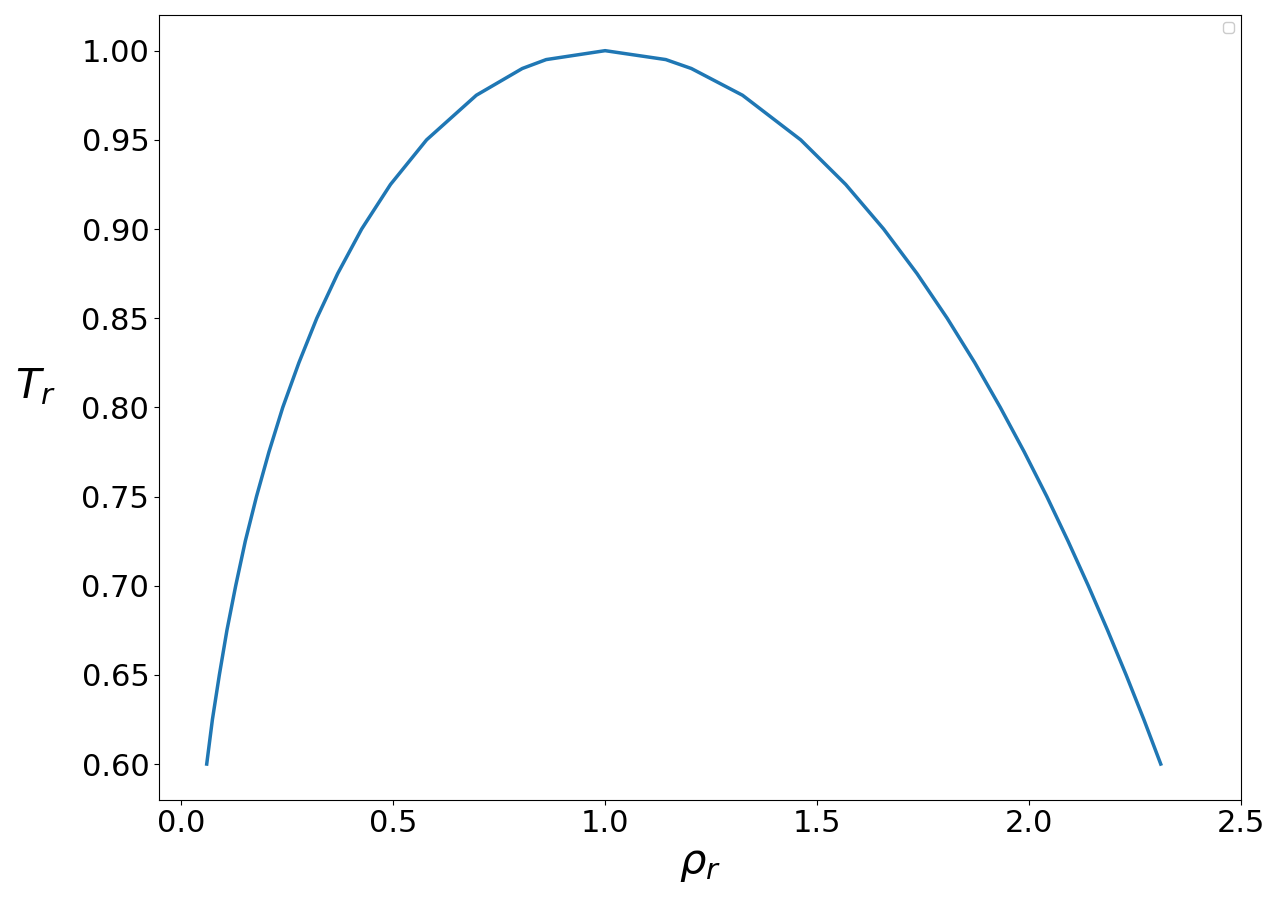
\includegraphics[width=.8\textwidth]{figs/cap4/Diagrama_T_r_vs_rho_r_analitico}
	\caption{Curva de coexistencia de fases para un fluido de VdW con los parámetros $a = 0,5 $ y $b = 4,0 $.}
	\label{fig:T_r_rho_r_analitico}	
\end{figure}

\newpage
Es de importancia destacar que las curvas de coexistencia dependen de la EOS que se esté utilizando para describir el comportamiento del fluido, en éste caso de estudio, la EOS es de VdW y posee  cómo parámetros \textit{a} y \textit{b} para describir los distintos fluidos .

\subsection{Validación}

Los valores que se utilizaron de $\Lambda$ y $\mathbf{M}$ para el modelo de LBM realizado se encuentran en el Apéndice (xxxx).

La validación de éste problema se hizo utilizando los parámetros $a =0,5$ y $b = 4,0$; para un tamaño de malla de 201 x 201 nodos y $T_r$ variando con un paso de $0,025$ en el rango de $[0,6 - 0,975]$. 
%La descripción de cómo se realizó la curva de coexistencia analítica se encuentra en el Apéndice (xxxx).

La Figura(\ref{fig:v_760_MxC_c_simple}) muestra la validación del código realizado en \textbf{C} para simple precisión; con distintos parámetros $\sigma$ del modelo MRT, donde se observa que el valor de $\sigma = 0,125$ es el que mejor ajusta a la curva de coexistencia. La Figura (\ref{fig:v_760_MxC_cuda_simple}) muestra el resultados obtenidos del código realizado en \textbf{CUDA C} en simple precisión.

\begin{figure}[h!]
	\centering
	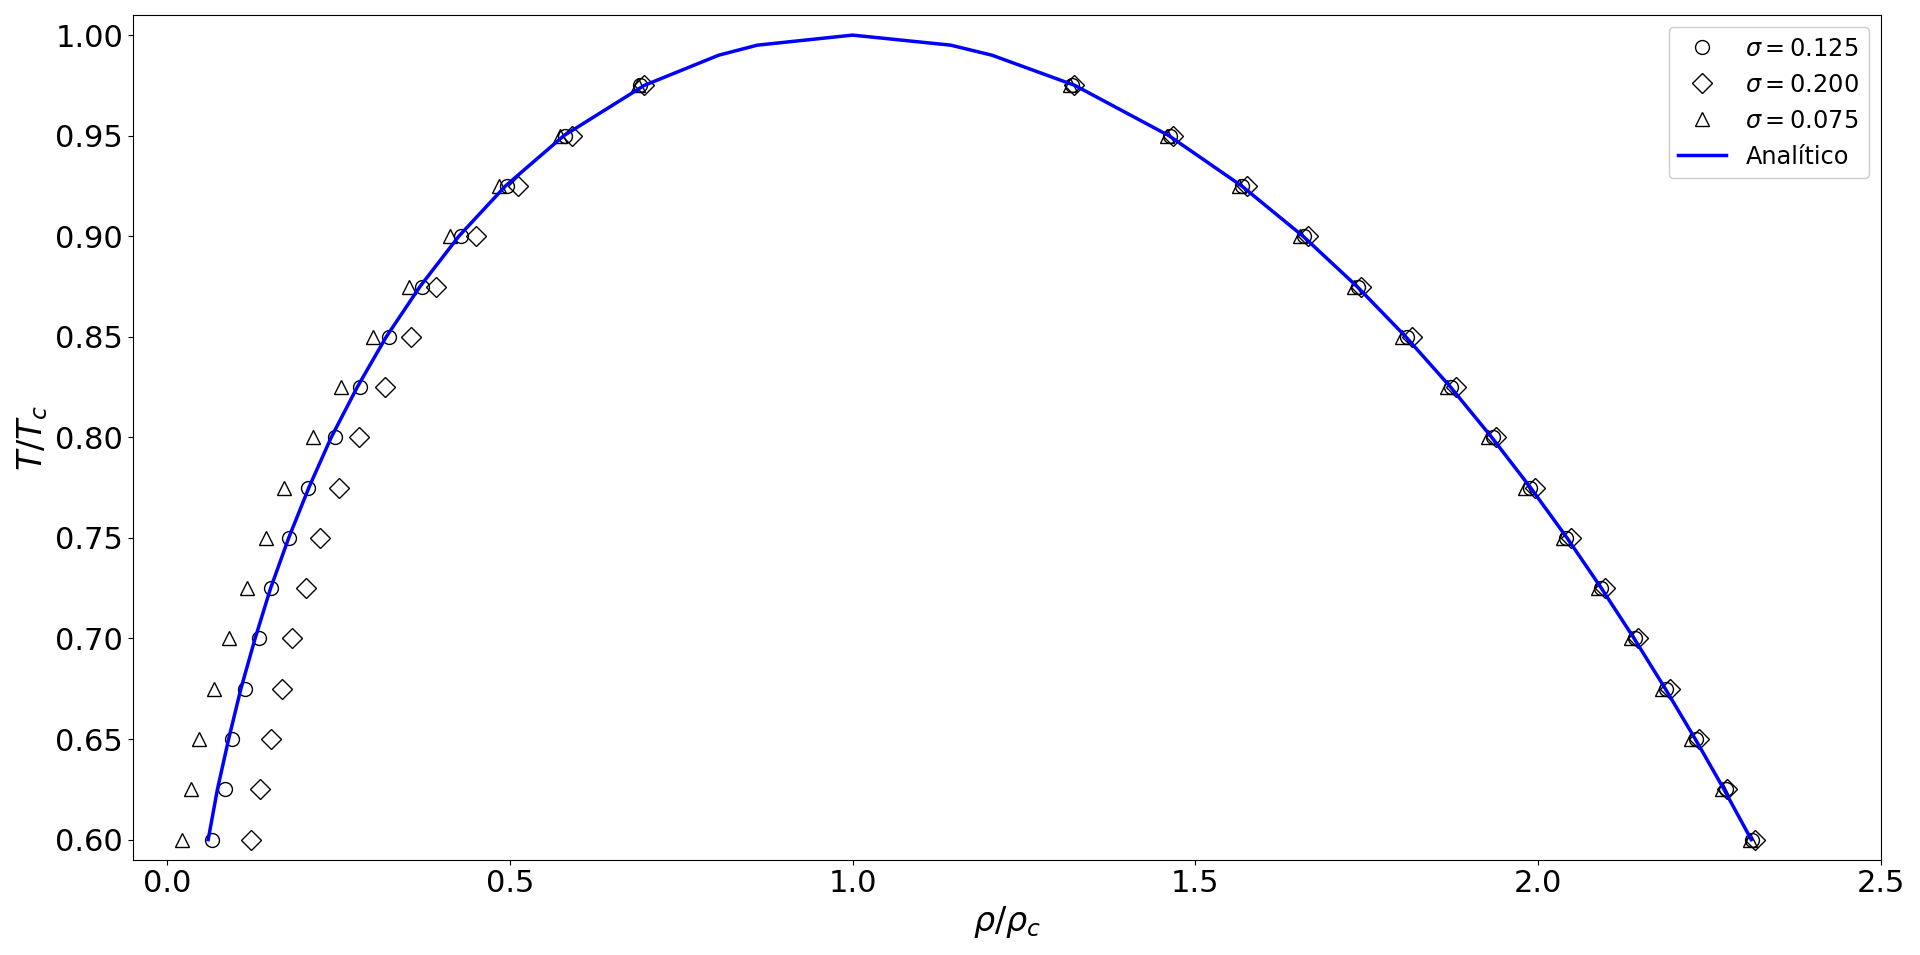
\includegraphics[width=\textwidth]{figs/cap4/v_760_MxC_c_simple}
	\caption{Curva de coexistencia de fases para un fluido de VdW con los parámetros $a = 0,5 $ y $b = 4,0 $, obtenida en simple precisión en la GPU NVIDIA Geforce GTX 760 en el código desarrollado en \textbf{C}. $\sigma = 0.075[\bigtriangleup]$	 $\sigma = 0.125[\bigcirc]$ y $\sigma = 0.200[\diamondsuit]$ }
 	\label{fig:v_760_MxC_c_simple}	
\end{figure}

\begin{figure}[h!]
	\centering
	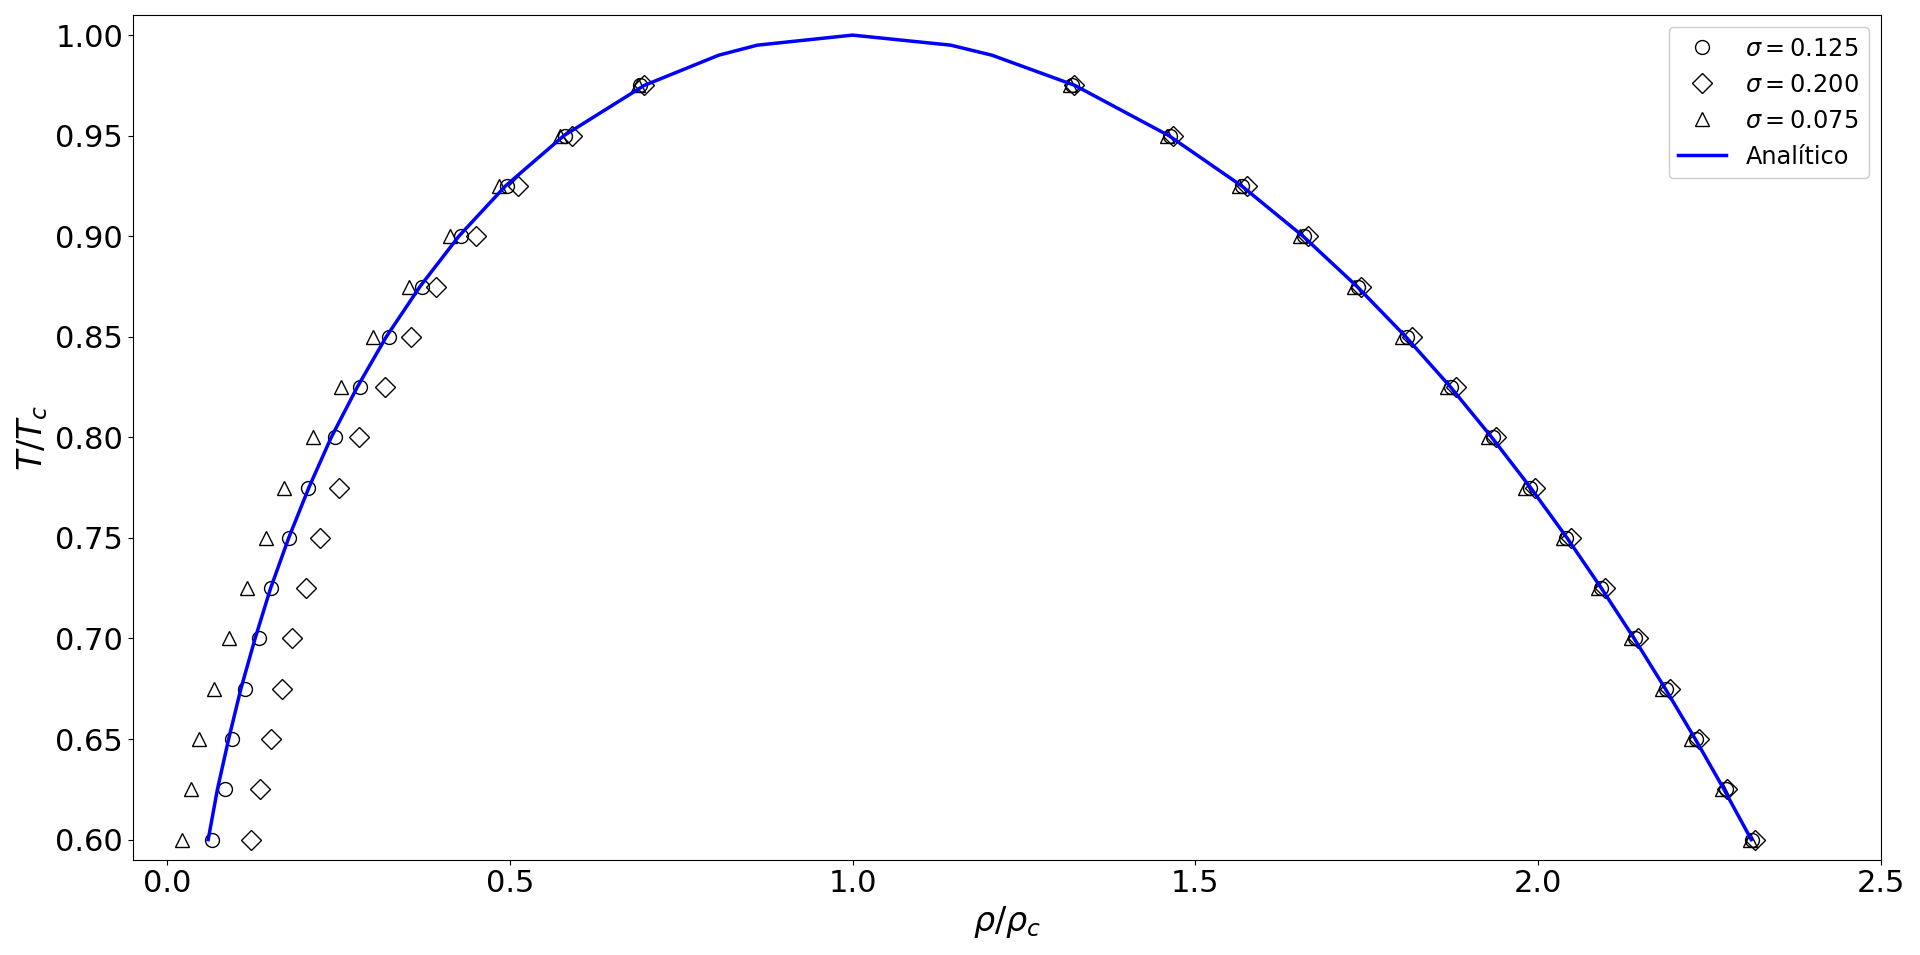
\includegraphics[width=\textwidth]{figs/cap4/v_760_MxC_cuda_simple}
	\caption{Curva de coexistencia de fases para un fluido de VdW con los parámetros $a = 0,5 $ y $b = 4,0 $, obtenida en simple precisión en la GPU NVIDIA Geforce GTX 760 en el código desarrollado en \textbf{CUDA C}. $\sigma = 0.075[\bigtriangleup]$	 $\sigma = 0.125[\bigcirc]$ y $\sigma = 0.200[\diamondsuit]$ }
	\label{fig:v_760_MxC_cuda_simple}	
\end{figure}

Ambos resultados mostrados en las Figuras (\ref{fig:v_760_MxC_c_simple}) y (\ref{fig:v_760_MxC_cuda_simple}) fueron realizados para 50000 pasos de tiempo en cada uno de los valores de $T_r$. El valor obtenido de las densidades de coexistencia de fases entre los códigos de \textbf{C} y \textbf{CUDA C} resultan exactamente iguales. 

El resultado que se obtuvo de realizar la validación en doble precisión es que los dos códigos desarrollados obtienen el mismo valor en las densidades de fase.

\newpage
\subsection{Comparación de precisión}
Se realizó la comparación de la precisión en cuánto diferian del resultado analícico esperado. Sabiendo que los código de \textbf{C} y de \textbf{CUDA C} brindan un resultado idéntico para simple precisión y doble precisión, solamente se muestra los resultados obtenidos en el código de \textbf{C}.

En cuanto a el resultado comparativo de las precisiones, la Figura (\ref{fig:v_760_MxC_c_comparacion}) muestra los resultados obtenidos en \textbf{C} para simple y doble precisión, siendo no apreciable a simple vista la diferencia.

\begin{figure}[h!]
	\centering
	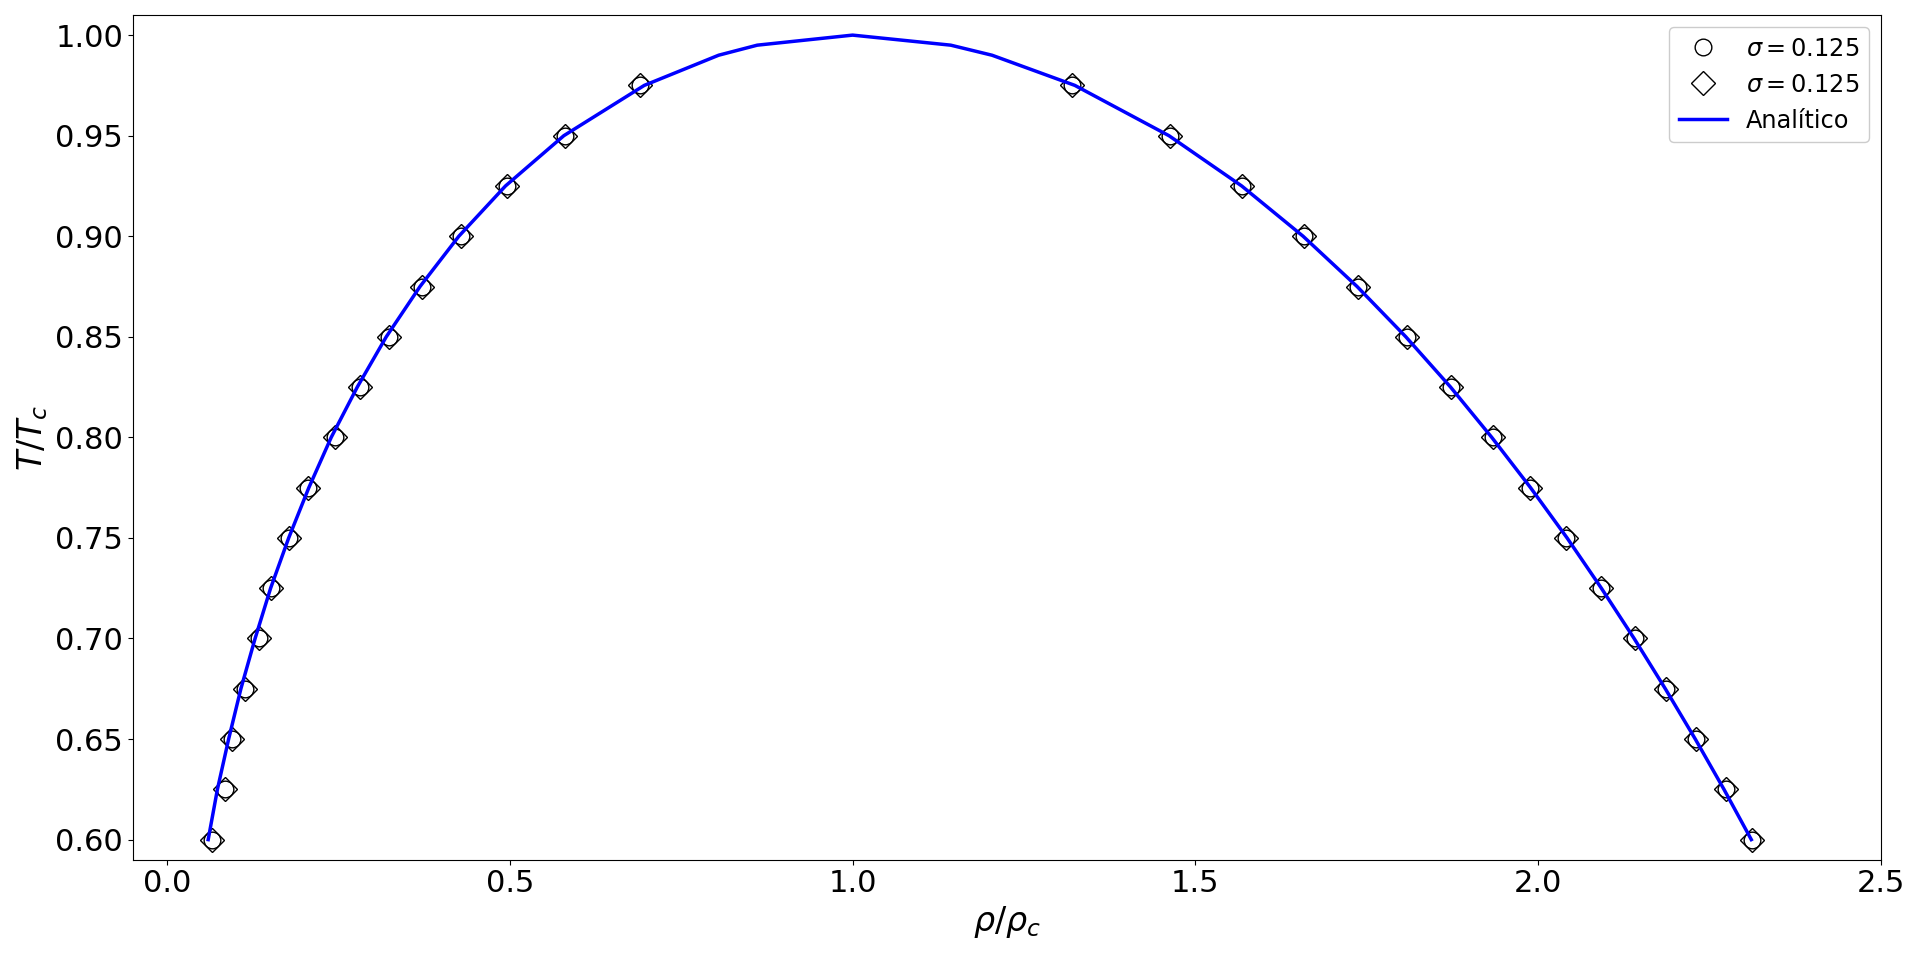
\includegraphics[width=\textwidth]{figs/cap4/v_760_MxC_c_comparacion}
	\caption{Curva de coexistencia de fases para un fluido de VdW con los parámetros $a = 0,5 $ y $b = 4,0 $, obtenida en simple precisión[$\bigcirc$] y doble precisión [$\diamondsuit$] en la GPU NVIDIA Geforce GTX 760 en el código desarrollado en \textbf{C}.} 
	\label{fig:v_760_MxC_c_comparacion}	
\end{figure}


La tabla \ref{tab:comp_MxC_precisiones_10} contiene los valores obtenidos para simple precisión y doble precisión. Se diferenció según el resultado obtenido de la densidad, si pertenece a la fase líquida o gaseosa, para realizar una comparación más detallada. Puesto que la fase líquida se ajusta mejor al valor analítico que la fase gaseosa.

Para realizar la comparación entre los resultados, se optó por hacerlo mediante comparación entre la norma euclídea (ver Ec.()) de los vectores de densidad analítica como el del resultado.

\begin{align}
	||a,b|| = \sqrt{\sum_i {\left( a_i - b_i \right)}^2  }
\end{align}

De


% Please add the following required packages to your document preamble:
% \usepackage{multirow}
\begin{table}[h!]
\centering
%\resizebox{17cm}{!}{
	\begin{tabular}{|c|c|c|c|c|c|c|}
	\hline
	& \multicolumn{3}{c|}{${\rho_{r}}_{\>gaseoso}$}      & \multicolumn{3}{c|}{${\rho_{r}}_{\>líquido}$} \\ \hline
	$\mathbf{T_r}$    & \textbf{Analítico}      & \textbf{Simple}       & \textbf{Doble}     & \textbf{Analítico}      & \textbf{Simple}     & \textbf{Doble}   \\ \hline
	0.600 & 0.0599097 & 0.0653772 & 0.0653724 & 1.32424  & 1.31956 & 1.31975 \\ \hline
	0.625 & 0.0733723 & 0.0848112 & 0.0847656 & 1.46149  & 1.46239 & 1.4624  \\ \hline
	0.650 & 0.0897449 & 0.0951336 & 0.095124  & 1.56762  & 1.56858 & 1.56859 \\ \hline
	0.675 & 0.107606  & 0.113153  & 0.113147  & 1.56762  & 1.65819 & 1.65821 \\ \hline
	0.700 & 0.128332  & 0.13353   & 0.133511  & 1.6572   & 1.73703 & 1.73704 \\ \hline
	0.725 & 0.150966  & 0.15182   & 0.151811  & 1.73595  & 1.80812 & 1.80813 \\ \hline
	0.750 & 0.177353  & 0.177323  & 0.177319  & 1.80706  & 1.87326 & 1.87328 \\ \hline
	0.775 & 0.206739  & 0.206086  & 0.206075  & 1.87233  & 1.93364 & 1.93364 \\ \hline
	0.800 & 0.23938   & 0.244229  & 0.244223  & 1.93243  & 1.98754 & 1.98759 \\ \hline
	0.825 & 0.277393  & 0.281299  & 0.281284  & 1.98899  & 2.04083 & 2.04085 \\ \hline
	0.850 & 0.319677  & 0.323471  & 0.323456  & 2.0423   & 2.09124 & 2.09124 \\ \hline
	0.875 & 0.368925  & 0.371915  & 0.371891  & 2.09234  & 2.14114 & 2.14117 \\ \hline
	0.900 & 0.425549  & 0.428416  & 0.428335  & 2.14012  & 2.18665 & 2.18665 \\ \hline
	0.925 & 0.493618  & 0.495973  & 0.495947  & 2.18563  & 2.23017 & 2.23019 \\ \hline
	0.950 & 0.493618  & 0.580402  & 0.580368  & 2.22933  & 2.27407 & 2.27411 \\ \hline
	0.975 & 0.578746  & 0.690126  & 0.690247  & 2.27117  & 2.312   & 2.312   \\ \hline
	\textbf{Distancia} & -         & 2.05233   & 2.05226   & -        & 0.14234 & 0.14241 \\ \hline
\end{tabular}%}
    \caption{Comparación de las precisiones con respecto a cuánto se acercan al valor analitico, tanto para doble, como simple precision, la norma utilizada para medir la distancia de los vectores es la norma  euclídea. Para el problema de la Construcción de Maxwell con la GPU NVIDIA Geforce GTX 760.}
    \label{tab:comp_MxC_precisiones_10}
    \end{table}







Uno de los objetivos de éste trabajo era ver también la diferencia entre las precisiones del código, cuánto difieren la simple precisión como la doble precisión y a su vez saber si es que hay una diferencia entre los tiempos que se tardan en ejecutar.

\newpage

\subsection{Speed Up}

En la presente sección se muestra cuánto es la mejora en el tiempo de cálculo realizado para el código de \textbf{C} y \textbf{CUDA C}. Se tomó una $T_r$ fija y se varió el tamaño de la grilla, de manera que ésta siempre fuese cuadrada.

La Figura (xxx) muestra los resultados obtenidos para un tamaño de grilla que va de 16 x 16 hasta 2048 x 2048, para diferentes número de bloques utilizados en la GPU, encontrándose el rango de 1 a 512, variando siempre de forma que el valor evaluado sea el doble que el anterior.
\\
\\
\\
xxxxxx insertar la figura de speed\_Up







\section{Estratificación de un fluido VdW con temperatura no uniforme}

Se quiere resolver el problema de, tener una cavidad unidimensional en presencia de un fluido cuya EOS es la de Van der Waals; con temperatura  no uniforme y fuerza de gravedad no nula. Éste problema fue desarrollado por Berberan-Santos \cite{berberan2002liquid} y que Fogliatto \cite{fogliatto2019simulation} extendió. 

Se toma como coordenada del problema \textit{y}, teniéndose una temperatura fija $T_{0}$ en $y = 0$ y $T_{1}$ en $y = H$ como se observa en la Figura (xxxx) que se muestra en presencia de la gravedad.





Se toma el problema de tener una cavidad unidimensional ocupada por un fluido cuya EOS es de Van der Waals, para temperatura no uniforme y fuerza de gravedad no nula.



\section{Generación de burbujas sobre una superficie horizontal calefaccionada}
%%% Local Variables: 
%%% mode: latex
%%% TeX-master: "template"
%%% End: 
